\chapter{Analysis and Design}
The focus of this chapter is to establish and discuss what the software is going to do and how it is going to achieve its intended goals. The defining actors were from different institutions related to the issues covered by the project. This chapter describes how they were involved as stakeholders, co-designers and evaluators. 

\begin{figure}[h]
\begin{adjustbox}{width=1\textwidth,center=\textwidth}
  \centering
  \includegraphics[scale=1]{images/stakeholders.png}
\end{adjustbox}
  \caption[Colaborators in the project]{Collaborators in the project.}
  \label{fig:stakeholders}
\end{figure}

\section{Users and stakeholders}

The following users were depicted for this development:

\begin{itemize}
    \item General public: Members of the general public who are concerned with the air quality of their environment.
    \item Pollution-sensitive public: People at risk of suffering health consequences due to air pollution.
\end{itemize}

To gain input from different perspectives, the following stakeholders were involved in the development: 

\begin{itemize}
	\item Researchers 
    \begin{itemize}
      \item Asthma UK researchers: Meetings were arranged with various researchers from the Asthma UK group. They were involved early in the design of a first prototype, by providing ideas and highlighting issues that may arise from the perspective of a a medical researcher. The researchers were:  Dr Aziz Sheikh, director of the research group, as well as Dr Soyiri Ireneous, and Dr Lynn Morrice. They are also members of the Usher Institute of Population Health Sciences and Informatics\footnote{\url{http://www.ed.ac.uk/usher}}
      
    The following issues were raised in the meetings:
      \begin{itemize}
          \item Based on their experience further considerations should be taken into account when designing applications that rely on user input.
          \item Review past approaches/work to avoid known problems.
          \item An application should give actionable feedback rather than just displaying information.
          \item Ask the users in order to find out what they want.
      \end{itemize}
      \item University of Edinburgh School of Informatics researchers: My supervisor Dr Ewan Klein and Catherine Magill, who are both researchers at the University of Edinburgh and part of the Edinburgh living lab which focus is on open data and how it impacts on behaviour and society. They also have a strong background in participatory design and were asked to provide feedback on inner prototypes.
	\end{itemize}
	\item Domain experts    
   \begin{itemize}
      \item Chief Technology Officer: Simon Chapple as CTO of Datalytics technology, a company with expertise in developing mobile applications for a different range of platforms. His opinion was valuable on technical or design issues that may arise in the development. He was asked for feedback about the design of a prototype of the application.
    The following recommendations were raised in the meeting:
    \begin{itemize}
        \item User interfaces should aim to be self-explanatory. 
        \item Colours should be consistent and provide meaning, as users associate colours to real world entities.
        \item Further consideration should be taken when choosing a native vs. hybrid development approach.
        \item Welcome screens should have an immediate, understandable objective.   
    \end{itemize}
\iffalse
\item How to ref this?: Mic starbuck, an activist who is involved in the guverment council and suffers from asthma was involved in the very first ideas of the design of the application, from his input, we were able to understand in a broad sense, what might an asthma sufferer need. (PEND)
\fi
\end{itemize}
    
%"I wonder how you did the animations behave that way"
    \item Users as stakeholders: The final users were involved in three stages. In the requirements elicitation, as co-designers for the prototypes and as evaluators of the final product. 
    \begin{itemize}
            \item Asthma UK patient group: They represent a sample of pollution-sensitive users. They are potentially a good source of data because they are already aware of the issues around air quality. They were involved in two phases: requirements elicitation, which was carried out via an online questionnaire, and the evaluation of the third final prototype.
            \item University of Edinburgh students: They represent a sample of the general population and were involved in three phases: the requirements elicitation, which was carried out via an online questionnaire, the evaluation of inner prototypes and the evaluation of the third final prototype. 
    \end{itemize}
\end{itemize}

\section{Requirements elicitation}
According to Somerville there are two kinds of requirements \cite{Sommerville2010}:
\begin{displayquote}
\begin{itemize}

\item Functional requirements: statements of services the system should provide, how the system should react to particular inputs, and how the system should behave in particular situations

\item Non functional requirements: Constraints on the services or functions offered by the system.... often apply to the system as a whole, rather than individual system features or services.


\end{itemize}
\end{displayquote}

The main functional requirements were elicited from the users because they were the first reason of the development. This was done through an online Survey Monkey questionnaire,\footnote{\url{https://www.surveymonkey.com/results/SM-Z7HH28LM/}} sent to Asthma UK volunteers and to students from the University of Edinburgh. Feedback from researchers and domain experts was taken into account as non-functional requirements as they did not ask for any particular function per se but just established some guidelines and features they believed would strengthen the application.

\subsection{Survey}

When designing the questionnaire there was an interest in knowing about existing air quality data sources used by both kinds of users and what did they find useful from them. They were also queried on how often they were using the information sources, their ages, and their needs for a new air-quality application.

There were 11 responses in total, 8 from the patient group and 3 of them from the general public. The ages of the respondents were varied: three between 25-34, 3 between 65-74, 2 between 18-24, 2 between 35-44 and 1 between 55-64 years old as shown in the figure \ref{fig:survey_ages}. 

\begin{figure}[H]
\begin{adjustbox}{width=1\textwidth,center=\textwidth}
  \centering
  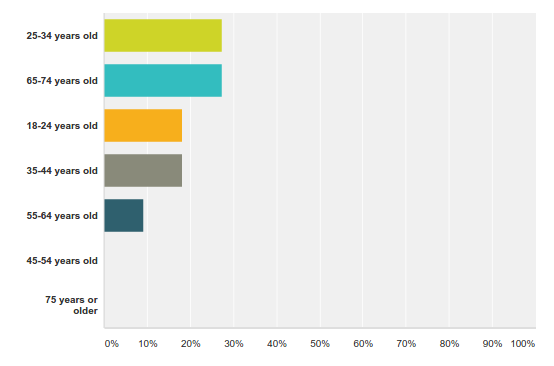
\includegraphics[scale=1]{images/ages_survey.png}
\end{adjustbox}
  \caption[Survey respondents ages ]{Survey respondents ages}
  \label{fig:survey_ages}
\end{figure}

Regarding previous usage of air quality sources, only half of the pollution-sensitive respondents were able to name the websites or applications they were currently using, while all the non-sensitive respondents named at least one source of information. Also, the sensitive respondents who reported the use of air quality sources tended to use them on a more regular basis than non-sensitive users. Reflecting on these answers: sensitive users may be inclined to require a support tool on a regular basis, but not all of them are aware of its existence.

The main findings from the survey were the potential new functionalities that users would like in a new Air Quality application, suggesting that there are unaddressed needs from current AQ sources. These are the main focus of the development of a new AQ application. From Figure \ref{fig:survey_new_features} we can see that the most important need is to visualise different individual pollutants, as current approaches often fail on treating them individually and thus enable respective decisions on this information. The second most important unaddressed need is to be able to personalise the air quality advice given a user's personal circumstances. The third most important requirement is to compare and visualise individual pollutants over different periods of time. 

Another interesting outcome was whether including tools to allow users to keep track of their symptoms would be of interest. Just three of the eleven queried persons responded positively suggesting that they may feel it unnecessary or tedious to input their symptoms on a regular basis.


\begin{figure}[H]
\begin{adjustbox}{width=1\textwidth,center=\textwidth}
  \centering
  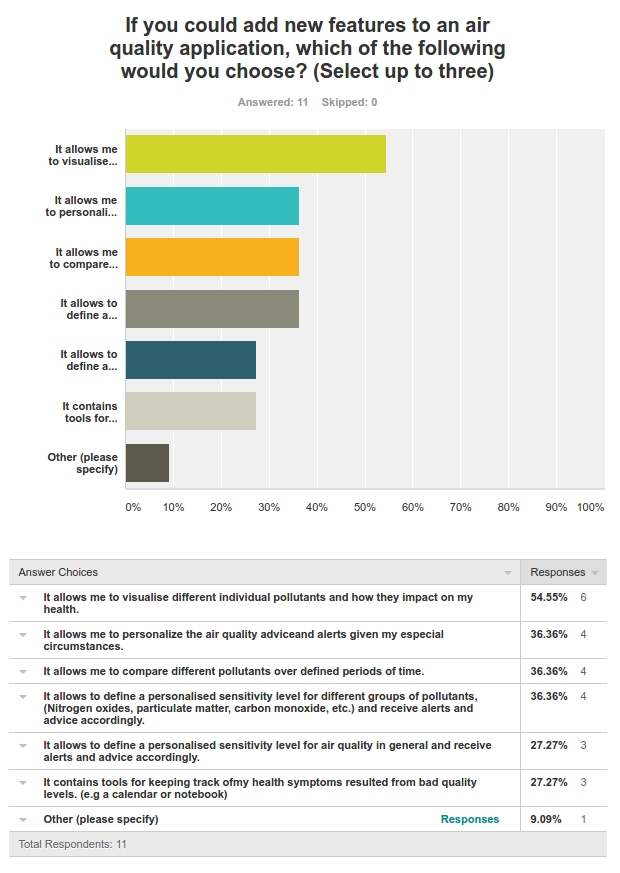
\includegraphics[scale=1]{images/new_features.png}
\end{adjustbox}
  \caption[New features for an AQ application]{New features for an AQ application}
  \label{fig:survey_new_features}
\end{figure}

\subsection{Interviews}
 
Meetings were held with the aforementioned researchers and domain experts to receive input from different points of view. At an early stage of the design process, the first person who showed interest was Mic Starbuck. From his perspective as a person suffering from asthma he mentioned the need for a tool to be able to visualise the relative impact upon a person's health based on different factors: like a person's health status, location, altitude and individual pollutants. He also mentioned that he browsed the web frequently to understand how AQ is behaving at different points of the day to decide whether to go outside for certain activities. 

Later in the process, the Asthma UK Centre for Applied Research (AUKAR) showed interest and a meeting was arranged. It took place with Dr Aziz Sheikh, Lynn Morrice, Dr Soyiri Ireneous and Catherine Magill. They expressed interest in collaborating with this project as well as participating closely to the School of Informatics in future research. They were presented with mock-ups of an application with visualisation and tracking purposes. However, based on previous work on tracking asthma status they pointed out that applications that rely on user input may not be successful because they demand too much from the user. For instance, much effort would be required to develop interfaces suited for particular users and their sets of circumstances. From this more focus was put into visualisation and recommendation capabilities than tracking.

Another meeting was held with Dr Soyiri Ireneous, an asthma researcher, and Catherine Magill. The purpose of this session was to understand in more depth the consequences of air pollution upon a person's health and how they might be presented in an air quality application. The possibility of including health advice was discussed. Data  with an easy to follow health guide is more valuable than data alone because the user can immediately know what to do under special circumstances. Also, Dr Soyiri as a mobile phone user, was concerned with the speed of the application as well the memory and battery usage.

\subsection{Functional requirements}

As time was limited the development covered the first three and most important needs set out by the final users. The following list summarises the final formal functional requirements for the development:

\begin{itemize}
    \item Being able to visualise the air quality status in general.
    \item Being able to visualise individual pollutants status and information on how they impact on a person's health.
    \item Being able to visualise individual pollutants over time.
    \item Being able to receive advice on the air pollution based on the variables like location, age and pollution sensitivity. 
    \item Being able to personalise the received advice indicating the personal pollution tolerance or sensitivity.
\end{itemize}

\subsection{Non functional requirements}

Summarising from the meetings, the following were established as non-functional requirements:

\begin{itemize}
    \item Is adequate for mobile devices (\textbf{Mobility}).
    \begin{itemize}
        \item Does not consume much storage space.
        \item Does not consume much battery.
        \item Is compatible with multiple devices.
    \end{itemize}
    \item Is usable (\textbf{Usability}):
    \begin{itemize}
        \item Easy to learn.
        \item Attractive to use.
    \end{itemize}
    \item Is efficient (\textbf{Performance}).
    \begin{itemize}
        \item Starts rapidly
        \item Loads and displays visualisations fast
    \end{itemize}
\end{itemize}


\section{System architecture}
In order to accomplish the requirements, it is important to consider design choices that could contribute towards qualities that are more adequate for this kind of development. For this, a trade-off between the three qualities of the software will be considered as shown in Figure \ref{fig:balance_attributes}, as it is not always possible to have everything in a system due to the possible conflict of attributes. For example, a highly animated and attractive design would affect the performance of the system and its capability in accomplishing the primary goal. Architectural choices will be taken into account over trade-off.


\begin{figure}[H]
\begin{adjustbox}{width=.5\textwidth,center=\textwidth}
  \centering
  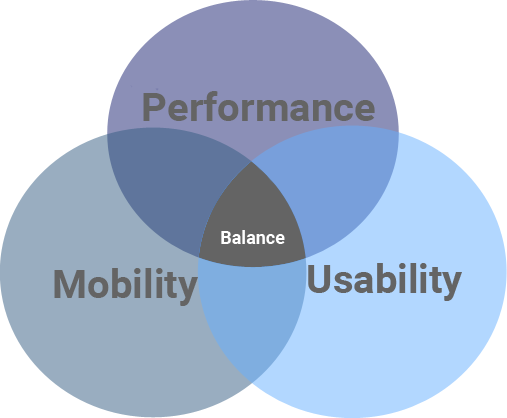
\includegraphics[scale=1]{images/balanceCircles.png}
\end{adjustbox}
  \caption[Finding a balance between software attributes]{Finding a balance between software attributes}
  \label{fig:balance_attributes}
\end{figure}

\subsection{Development approach and operating system}
It is possible that the development could take a hybrid or a native approach, as summarised in Table \ref{tab:development_approaches}. In a nutshell, it means that the software could be developed in a web-browser container and therefore be compatible with all devices able to display modern web-pages. Or it could even be be developed using the native software development kit for each system (Android, iOS, etc) therefore making it compatible with that specific operating system. A native development approach carries with it the disadvantage that a new source code would be needed for each operating system. Alternatively it would bring many benefits such as the response speed, being able to use advanced graphics and animation techniques and having an easy access to the native APIs and components of the device (e.g. GPS and gyroscope). In order to gain performance and usability a native approach has been chosen. Consequently, it is important to define the operating system target, which will solely be based on the market share of the most important operating systems according to IDC. \footnote{\url{http://www.idc.com/prodserv/smartphone-os-market-share.jsp}} Android holds a commanding share of 82.8\%, compared to 13.9\% of iOS, and 2.6\% for the Windows phone. Because of this, to target a wider range of mobile phone users the selected operating system for developing the application is Android.

\begin{table}[ht]
\centering
\begin{adjustbox}{width=.6\textwidth,center=\textwidth}
\begin{tabular}{lrr}
  \hline
   - & Native & Hybrid  \\ \hline
   Language & Switf or Java & HTML and Javascript \\
   Speed & Fast & Medium \\
   Portability & None & High \\
   Advanced Graphics & High & Moderate \\
   Access to native APIs & High & Moderate \\
   Development cost & Expensive & Reasonable \\
   \hline
\end{tabular}
\end{adjustbox}
  \caption[Native vs hybrid development approach ]{Native vs hybrid development approach. (Adapted) \footnotemark }
\label{tab:development_approaches}
\end{table} 
\footnotetext{\url{http://julyrapid.com/hybrid-vs-native-mobile-app-decide-5-minutes/}}

\subsection{Air quality data source}
It was considered to acquire personal air quality sensors to provide real-time high-resolution data to the system; unfortunately, such devices are still not very feasible as they are costly and become obsolete over time due to loss of accuracy. One example is the Libelium Gases PRO sensor, which costs around \euro{}2000 and has an approximate lifetime of 12 months\footnote{\url{http://www.libelium.com/calibrated-air-quality-gas-dust-particle-matter-pm10-smart-cities/}}. 

As mentioned in the background, there are currently many automatic fixed sensors around Scotland that include a variety of pollutants and provide real-time data. However, the data of these devices is not exposed through any public API from the Scottish government but as plain HTML. One possibility as well is using any third party air quality data source such as the Breezometer air quality API\footnote{\url{https://breezometer.com/air-quality-api/overview/}} or the OpenAQ API\footnote{\url{https://openaq.org/#/}}. The first one is a private source of air quality data which bills for the queries to the service and thus not very cost-effective. The second is a public API but the number of sensors from each city in Scotland are limited compared to the official government sources. An example of this is the city of Glasgow, which from the official sources has 26 fixed automatic sensors but from the public API only 4 are available. As a result, to have a more accurate air quality source the data will be collected from the official sources and exposed to later query from the device. 


\subsection{Infrastructure as a service}

IaaS or Infrastructure as a Service is a cloud service that provides computing infrastructure on demand. The benefits of using such a service as opposed to traditional approaches are many. First, there is no need to buy, install and maintain a server at a fixed location, reducing associated costs. Second, setting up an IaaS can be done within minutes, saving  development time. The following options were considered for setting up an IaaS: 

\begin{itemize}
	\item Google Cloud Platform \footnote{\url{https://cloud.google.com/}}
    \item Amazon Web Services \footnote{\url{https://aws.amazon.com/}}
    \item Microsoft Azure \footnote{\url{https://azure.microsoft.com/en-us/}}
\end{itemize}

Due to budget constraints, the most cost-effective solution was chosen. Amazon's free tier allows up to 12 months of free usage, as opposed to Microsoft's 30 days trial and Google's 60 days trial.

\subsection{Back-end technological choices}
The back-end component of the system will perform two functions: 

\begin{itemize}
	\item Gather the required air quality data and insert it into a database. The easiest way to do this is via any available web-crawling libraries, such as Jspider\footnote{\url{http://j-spider.sourceforge.net/}} for Java or Scrapy \footnote{\url{http://scrapy.org/}} for Python. Scrapy was chosen because it is a complete and stable framework that can handle crawling operations in an easy way. 
	\item Provide service to the mobile application. There is a need for a logic tier to process the input elements for the health advice. As Java is a stable and reliable framework,  it is well suited for most of the tasks that require server side processing and client handling in an optimal way.
\end{itemize}

\subsection{Schema-free database}

Air quality readings will need to be stored for later query from the device. For this, there is the option of using standard SQL databases or schema-free databases. Analysing the data that will be stored in further detail, it will contain the readings gathered from each sensor in Scotland, and specific information such as their name, location and type of sensor. The data would be extracted in the form of JSON documents without normal relations between them. Moreover, the transactions between the devices and the database should be as fast as possible without immediately considering instant reliability as sensors are updated at best each hour. Another advantage of these types of databases is the agility they provide by eliminating the need of schemas. Taking into account these factors, it is more suitable to use a schema-free database or NoSQL. Specifically, it will be used a Dynamo NoSQL from the same Amazon Web Services infrastructure because it integrates easily with the already chosen IaaS.

\subsection{Overall design}
The overall design of the infrastructure is as shown in Figure \ref{fig:architecture}. The back-end and the database components run on Amazon Web Services (AWS). The Android device uses the AWS Software Development Kit (SDK) to make queries to the Dynamo database directly to read the air quality data, this to facilitate the mapping between the objects in the database and the Android device. To access the advice service, the approach is to make HTTP GET requests to the Java containers hosted in AWS. 
\begin{figure}[H]
\begin{adjustbox}{width=.65\textwidth,center=\textwidth}
  \centering
  \includegraphics[scale=1]{images/architecture.png}
\end{adjustbox}
  \caption[Architecture design]{Architecture design}
  \label{fig:architecture}
\end{figure}

\section{Mobile application}
The Android application will be the visible interface for the final user. At this point it is key to understand the design choices that can affect our main quality attributes. These are the development of the user interface and the lower-level issues related to the management of the screen components.

\subsection{User interface}
Three distinct screens will achieve the functional requirements as shown in Figure \ref{fig:chain_of_screens}. The first screen will be responsible for displaying a general overview and personalised advice. The second screen will show individual pollutants and the third individual pollutants over time. There will be another initial screen to allow users to input the personal details needed for the application.

One useful guideline at the design level to connect the screens with each other is simplicity. Having many different screens for different purposes could overwhelm the user, so they will be accessible at every time using a tabbed menu and enabling gestures to navigate through them. That is, the screens will become active by selecting a tab, or by swiping between them.

\begin{figure}[H]
\begin{adjustbox}{width=.45\textwidth,center=\textwidth}
  \centering
  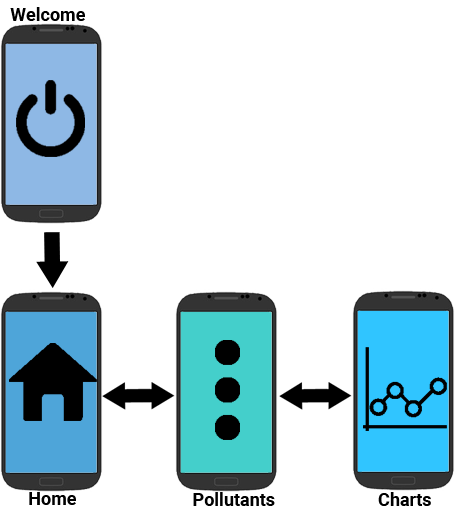
\includegraphics[scale=1]{images/screenChain.png}
\end{adjustbox}
  \caption[Chain of screens]{Chain of screens}
  \label{fig:chain_of_screens}
\end{figure}

\subsection{Activities}
The previous screens will be developed individually by the use of activities. An Activity is the abstraction employed by the Android framework to contain the visual and run-time elements of the currently displayed screen. The way Activities are created and maintained in the screen is quite unusual in contrast with standard Java Swing interfaces. It makes use of an event driven life-cycle that must be understood beforehand for a smooth and error-free behaviour. 

As available RAM is limited on a handheld device and it has to be shared with all other running applications, it is not possible to maintain all activity instances in memory. The activity lifecycle is a workaround for this problem, allowing the Dalvik virtual machine (A virtual machine that runs all Android programs) to determine automatically which activities will be kept in memory. Thus, the activities should provide behaviour to be called from any point in the lifecycle.

The lifecycle is illustrated in Figure \ref{fig:activities_lifecycle}. It can be observed that the first method called by Android is the \textit{onCreate()} method, used to instantiate the requested activity and any screen components. Later, the application can pass to other states until it is stopped and started again from a different entry point to the one it was previously created from. The activities should be able to handle both starting points and restore any state left by the user when the activity was stopped. 

\begin{figure}[H]
\begin{adjustbox}{width=1\textwidth,center=\textwidth}
  \centering
  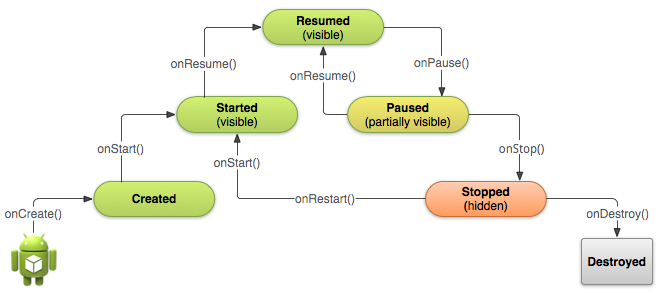
\includegraphics[scale=1]{images/basic-lifecycle.png}
\end{adjustbox}
  \caption[Android activities lifecycle]{Android activities lifecycle\footnotemark}
  \label{fig:activities_lifecycle}
\end{figure}
\footnotetext{\url{https://developer.android.com/training/basics/activity-lifecycle/starting.html}}

\subsection{Layouts}
The main component to render a screen in Android is the Layout. Layouts make use of XML to define the objects on the screen. As shown in the example below, it renders a \textit{TextView} object followed by a \textit{Button} object. Layouts need to be attached to an activity or fragment to give them behaviour. Once attached, the components defined by the Layout can be extracted by using their ID's and the method \textit{findViewByID}
\begin{verbatim}

<?xml version="1.0" encoding="utf-8"?>
<LinearLayout xmlns:android="http://schemas.android.com/apk/res/android"
              android:layout_width="match_parent"
              android:layout_height="match_parent"
              android:orientation="vertical" >
    <TextView android:id="@+id/text"
              android:layout_width="wrap_content"
              android:layout_height="wrap_content"
              android:text="Text" />
    <Button android:id="@+id/button"
            android:layout_width="wrap_content"
            android:layout_height="wrap_content"
            android:text="Text" />
</LinearLayout>
\end{verbatim}

It is important to understand the correct coupling of Android layouts because this influences how fast the screen is rendered. The rendering process is called \textit{inflating} and occurs in the \textit{onCreate()} method. As the Activities are rendered on the screen, children components are attached and may call to render their own layout, potentially slowing down the the application. For this purpose, the Android SDK makes available the Android device monitor to understand how much time is being taken to render all the components displayed at a given time. 

The Android device monitor helps to visualise the components taking part on the screen at some point in run-time. It shows  the topmost (the root) to the bottommost element (the leaf), how they are attached and which element of the entire tree is taking the most time to render, therefore helping in the debugging process. As shown in Figure \ref{fig:android_device_monitor}, the delaying components are marked with red dots which means that the rendering of that specific screen component is among the slowest half of views. The yellow means the view renders faster than the bottom half of the other views and the green means that renders faster than at least half of the other views. Understanding this tool helps achieving the required performance quality attribute. 

\begin{figure}[H]
\begin{adjustbox}{width=1\textwidth,center=\textwidth}
  \centering
  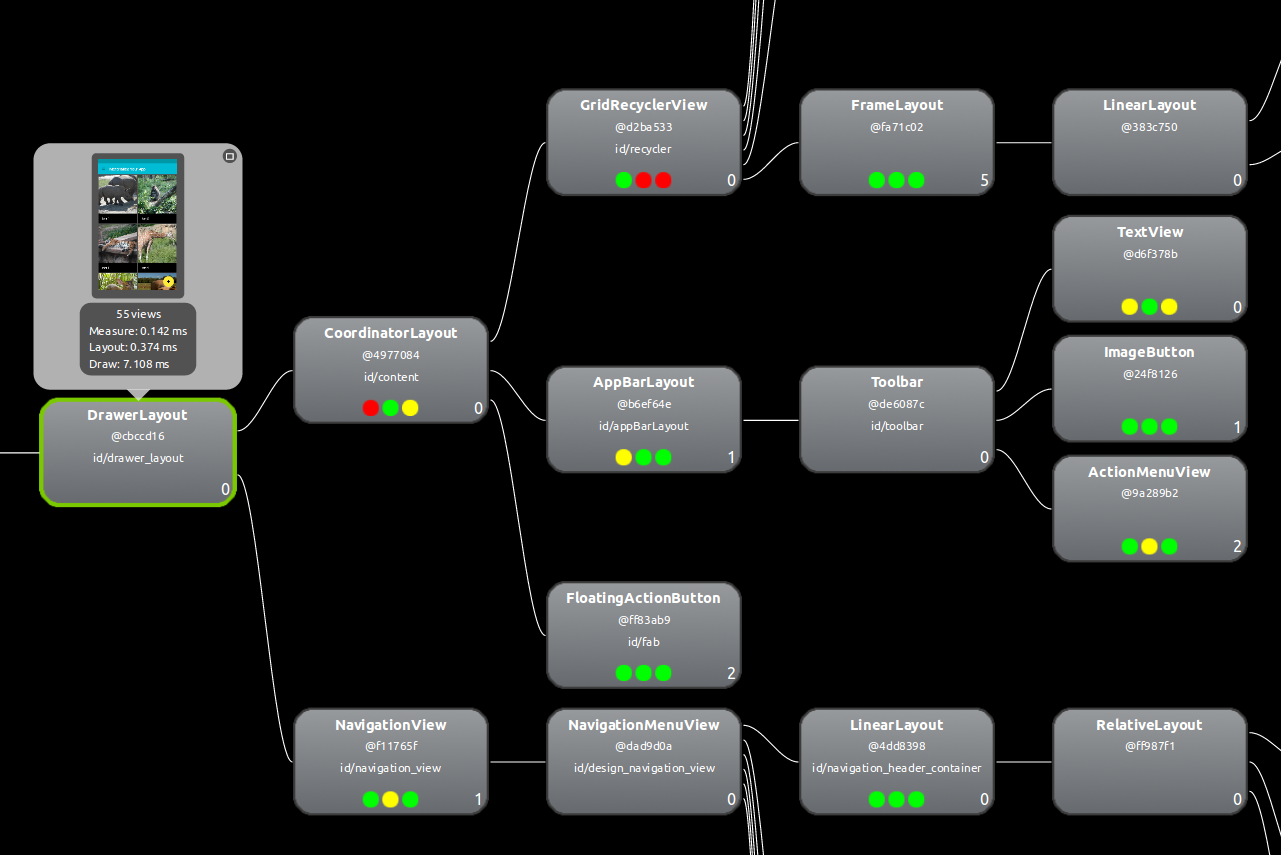
\includegraphics[scale=1]{images/android_device_monitor_2.png}
\end{adjustbox}
  \caption[Android device monitor]{Android device monitor}
  \label{fig:android_device_monitor}
\end{figure}

\subsection{Material design}
As well as understanding how to achieve a smooth behaviour within the application it is wise to revise the good use of design principles available to enhance usability and its implied attributes, ease of use and attractiveness.

According to Google: \begin{displayquote}Material design is a visual language for our users that synthesises the classic principles of good design with the innovation and possibility of technology and science. \end{displayquote} 

The material design framework helps with principles that address design issues to allow every application user to navigate, understand and use the designed user interface (UI) successfully. It also serves to unify the experience across different devices and screen sizes, so that users will be able to understand naturally design cues of new applications. The following principles are adhered to: 

\begin{itemize}
    \item Material: The material metaphor is based on paper and ink like in the real world, in three dimensions using lights and shadows. The intention is to close the gap between the perception of real world elements and digital elements. 
    \item Graphics: The use of graphical elements such as typographies, icons, adequate colours and images make a pleasant interface and give hierarchy and meaning. 
    \item Motion: User actions that initiate motion and transform the state of the interface serve as playful cues that help to understand the flow of the interface as well as to provide continuity and feedback. 
\end{itemize}


\begin{figure}[H]
\begin{adjustbox}{width=1\textwidth,center=\textwidth}
  \centering
  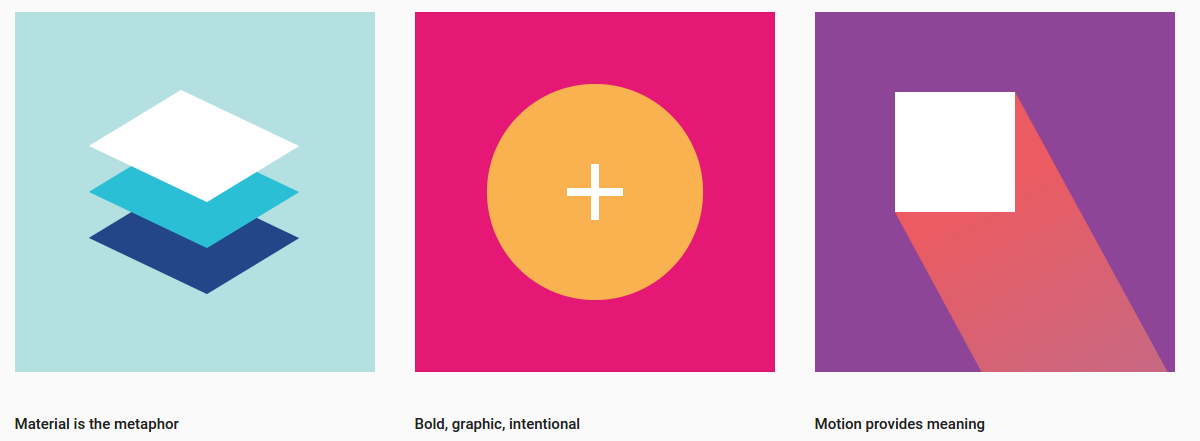
\includegraphics[scale=1]{images/material_google.png}
\end{adjustbox}
  \caption[Material design framework]{Material design framework \footnotemark}
  \label{fig:android_material_design}
\end{figure}
\footnotetext{\url{https://material.google.com/}}

\subsection{Targeted devices}
As the Android OS and APIs (Application Programming Interfaces) are updated over time some applications built with later SDK versions will not be compatible with earlier OS versions. Thus, it is important to define the earliest operating system that will be included in the development. For this, considerations such as the number of users that are still using old versions of Android and new features that might be useful from newer SDK versions should be studied. For instance, the most used OS distribution nowadays is KitKat which makes use of an API level 19 as shown in Figure \ref{fig:android_platform_versions}.  Unfortunately, it does not offer native support for material elements, which are a strong positive for this development. A workaround for this problem is to include the Android support library\footnote{\url{https://developer.android.com/topic/libraries/support-library/index.html}} which will provide compatibility for features made available in newer versions of Android. The final targeted API is level 19 (KitKat) for the use of an up to date stable API and to include up to the 79\% of the Android users.  

\begin{figure}[H]
\begin{adjustbox}{width=1\textwidth,center=\textwidth}
  \centering
  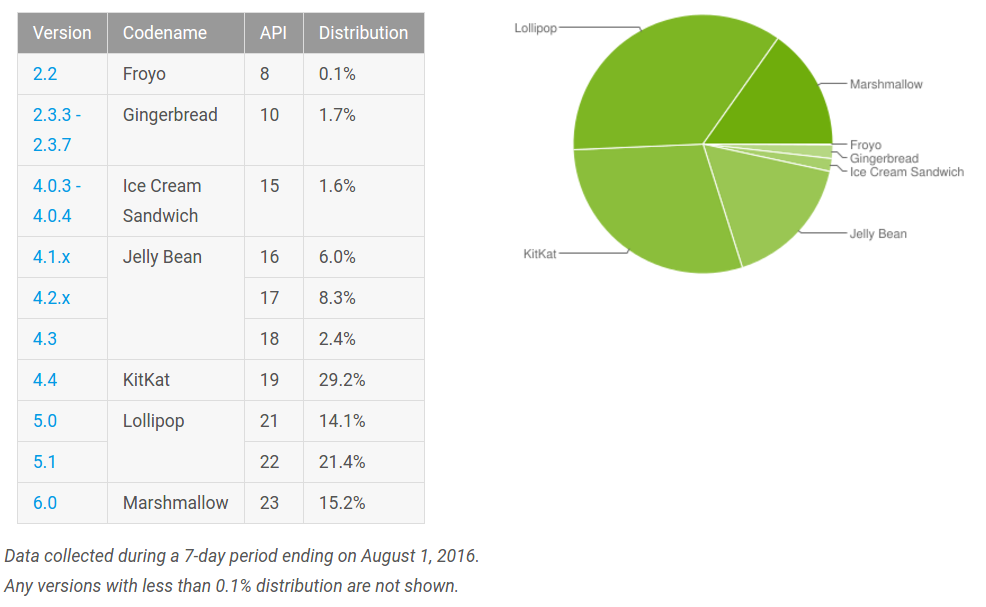
\includegraphics[scale=1]{images/android_platform_versions.png}
\end{adjustbox}
  \caption[Devices running a given version of Android]{Devices running a given version of Android \footnotemark}
  \label{fig:android_platform_versions}
\end{figure}
\footnotetext{\url{https://developer.android.com/about/dashboards/index.html}}

\section{Back-end}
Considering in detail, the back-end architecture will be composed as shown in Figure \ref{fig:architecture_back_end_detail}. A virtual machine will run Ubuntu Linux because it is a very stable and compatible version of Linux. There was also a possibility to use a custom Amazon flavour of Linux, which was not viable due software compatibility issues. The back-end will host two main components to power the application, the data service and the advice service. 

\begin{figure}[H]
\begin{adjustbox}{width=.6\textwidth,center=\textwidth}
  \centering
  \includegraphics[scale=1]{images/architecture_back_end_detail.png}
\end{adjustbox}
  \caption[Back-end architecture]{Back-end architecture detail}
  \label{fig:architecture_back_end_detail}
\end{figure}


\subsection{Data Service}
 The air data source is the air quality in Scotland website. As it displays the updated readings in HTML, a web crawler is needed to navigate the readings making use of XPATH selectors to extract the required data. Once extracted, it will be inserted in JSON format directly to the Dynamo database.
 
A daemon is a program that runs in the background autonomously and will call the web crawler every half hour to get the most up-to-date readings from the air quality readings. (They are updated at the most each hour). 

\subsection{Advice Service}
The advice service will be responsible for providing health advice based on the COMEAP report \cite{HealthProtectionAgencyfortheCommitteeontheMedicalEffectsofAirPollutants2011}. Before analysing the techniques that can be considered to translate the advice from the COMEAP report into a service, there are few matters to notice. The document has different categories of advice based on the sensitivity and age of the people. They are not simple data statements that can be easily used from a database, but more of logical statements. For example, from Figure 2.3 we can state that at-risk individuals, who are adults or children when the AQ index is from 7 to 9 points should reduce strenuous physical exertion. Also, it is likely that the health statements would need to be modified or expanded in the future. 

When it comes to providing logic or 'intelligence' to a system for it to make choices, such as the health advice, there are two general approaches that may be considered: rule-based systems and machine learning techniques. Rule-based systems or expert systems are a good fit when all the options for the system are known beforehand, and when all the conditions can be easily written as \textit{if else statements}. On the other hand machine learning techniques are useful when the datasets are fairly large and the rules have to be made at execution time. Therefore, the easiest way to provide the system with the capability to give the required health advice is via an expert system.

\section{First prototype}
Following the sketched application design and the interaction design methodology, the first prototype was drawn in order to meet the user requirements and to start defining how the final interface would look like. As mentioned, the application would be composed of three final distinct visualisations for the main functional requirements:

\begin{itemize}
    \item Visualise current air quality and provide health advice.
    \item Visualise individual pollutants status and information about their sources and effects.
    \item Visualise individual pollutants over time.
\end{itemize}


\begin{figure}[H]
\begin{adjustbox}{width=1.2\textwidth,center=\textwidth}
  \centering
  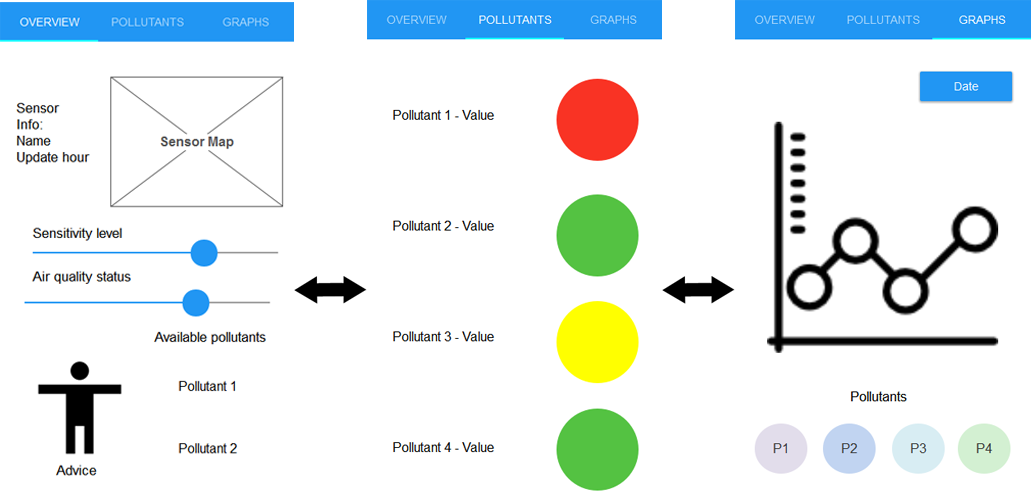
\includegraphics[scale=1]{images/firstPrototype.png}
\end{adjustbox}
  \caption[Frist prototype]{First prototype. From left to right: first, second and third visualisation}
  \label{fig:first_visualization_first_prototype}
\end{figure}


\subsection{Screen 1}

The first visualisation would contain first-hand pertinent information that would adhere to different functions. It would convey the current air quality status and its components, provide information about the source of the air quality reading, show air quality advice given the user configuration and finally let the user configure the air quality advice in a playful way. We could think of this screen as a dashboard that will give the user the required basic information to use the rest of the application. In fact, the display of this screen is enough to get a full picture of what is going on without much detail.
This screen is shown in Figure \ref{fig:first_visualization_first_prototype}. It is visually divided into the top and bottom component. The top component is information about the sensor so as to give the user confidence about the reading by means of a map, the hour it was last updated, and the name location of the sensor. The bottom component contains two bars: one for adjusting the sensitivity level, and the other to show the air quality status followed by the health advice in text and the pollutants at play in the reading at the point it was taken. 

\subsection{Screen 2}

The second visualisation aims to provide an individual visual hint for each pollutant. The need for this visualisation arises from the difficulty of to observe how the readings are at a pollutant level. The overall idea is to show a list of the pollutants that are present at the moment with a visual cue to allow for an immediate insight of the reading as well as containing the official measure and the measurement unit. Also, by clicking in each pollutant, it will be possible to examine more specific information about the pollutant.

\subsection{Screen 3}

The final visualisation will provide full detail of how the readings were behaving throughout the day, or on a particular date. The need for this visualisation arose from the need for sensitive users to relate their symptoms to pollution spikes and to gain knowledge about what might be affecting them at a pollutant level and support decision making. For this purpose, a line graph is employed as is an adequate tool to show readings over time. Also, the same pollutants that were taking part in the first and second visualisations will be consistent in this screen. The difference is that they will be touch-enabled to allow the user to select which pollutant to visualise as a way of providing interaction. At the top of the screen there will be controls to define the specific date and time of the readings.
